Our evaluation illustrates key findings about \sys. We show that: \todo{Make a list of core findings here once results are solid}{Przemek}

\subsection{\sys Runtime Performance}
\label{sec:results_evaluation}

We evaluated \sys to show that it is easy to use and efficient across our benchmarks. We evaluate \sys efficiency by comparing its runtime performance to Alpaca. We characterize \sys by studying how its performance varies due to coalescing.

\subsubsection{\sys Task Adaptation}
\label{sec:result_coalescing}

We first need to assess the performance of all coalescing strategies intriduced by us in Section~\ref{}.

\textbf{Coalescing Strategies.} Figure~\ref{fig:coalescing} shows the run time of \sys's two coalescing strategies normalized to the run time without
coalescing. We show data from experiments with intermittent power, where intermittency was generated in software
%\todo{Say briefly how we generate full reset with MSP430}{Amjad}
by triggering a reset from software at intervals that were uniformly distributed with an average power availability and unavailability interval of 15\,ms and 10\,ms respectively. Each application ran with the same generated pattern for the fairness of comparison. The results show the benefit from coalescing for most applications, with the
exception of dft, where wasted work dominated the gains from coalescing.
 %\todo{why coalescing for dft does not work but in Fig. 9 does?}{Amjad}
The difference in performance between HC and TSHC strategies is highly
application-dependent, with some applications benefiting from size awareness
while others suffering, due to decisions based on inaccurate prediction of the
actual task energy consumption. The TSHC gains are particularly small (or negative) for applications with narrower range of task sizes in Figure~\ref{fig:task_profiling}.
%\todo{say why this difference is small}{Amjad}.
%For this reason we shall proceed with HD coalescing strategy in subsequent evaluations. 

\begin{figure}
	\centering
	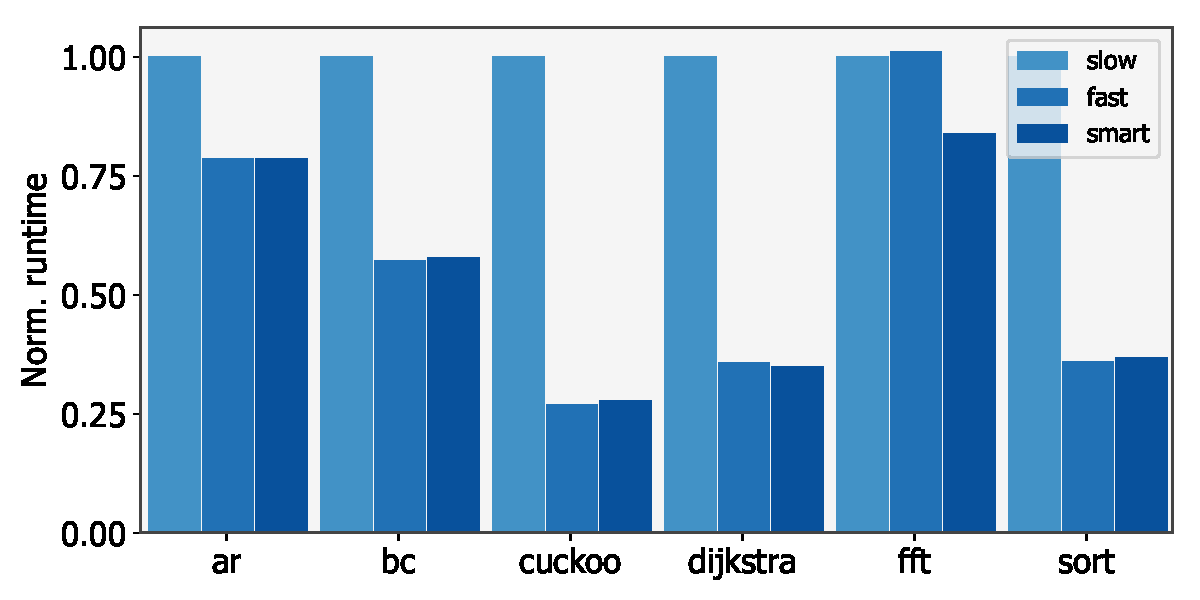
\includegraphics[width=\columnwidth]{figures/coalStrategies}
	\caption{\sys coalescing strategies performance per application on intermittent power compared to \sys without coalescing. \todo{Add new figure; comment on the result}{Przemek}}
	\label{fig:coalescing}
\end{figure}

\textbf{\sys versus Task-based Model.} We evaluate \sys's run time performance and compare \sys to the run time performance of Alpaca. Results are given in Figure~\ref{fig:runtime}. For each application we measured its execution time using real wireless power provision from the RF signal generator (refer to Section~\ref{}).

The data show the average execution time of each application run repeatedly for 20 seconds, with runtimes normalized to \sys's average. The results show that \sys provides a performance benefit compared to Chain for most applications. The performance benefit is greatest for applications that have small tasks (bc, sort, cuckoo) at all distances on intermittent power and with fixed power. In applications that have larger tasks (e.g. dft) or access more different memory pages, \sys incurs overhead from memory virtualization that cause its performance to be comparable to (or in the \emph{single} cem case, worse than) Chain. \todo{Rewrite conclusions}{Przemek}

\begin{figure}
	\centering
	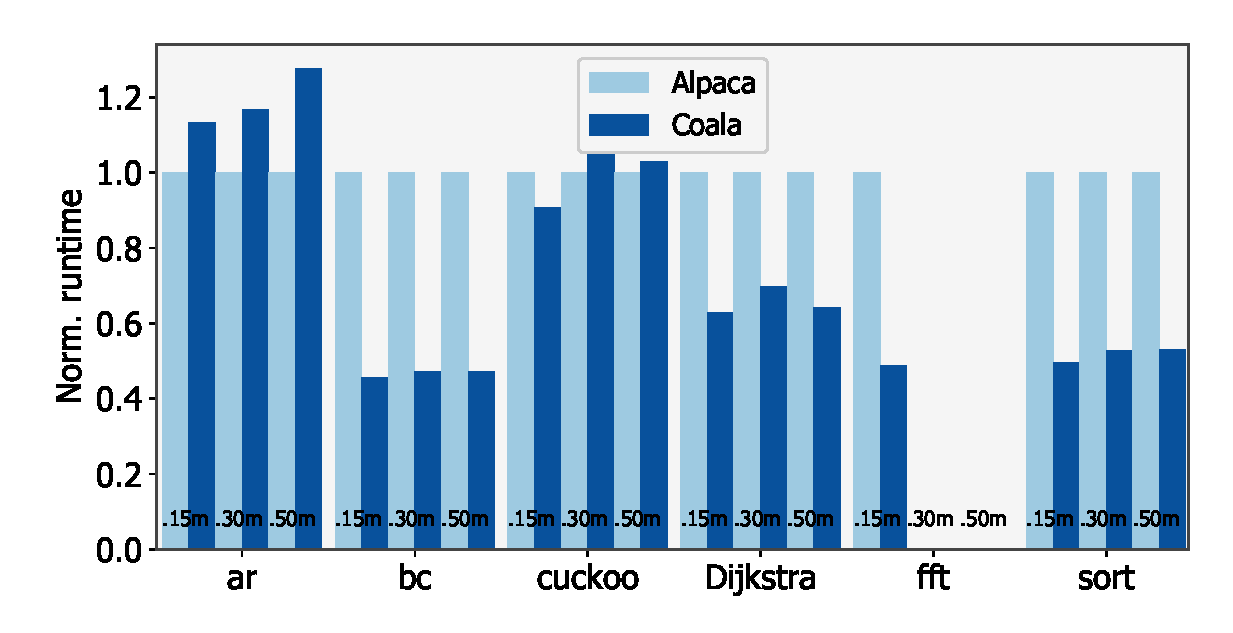
\includegraphics[width=\columnwidth]{figures/coala_alpaca_gcc}
	\caption{\textbf{Performance of \sys applications (divided manually into tasks) at multiple WISP to RFID reader antenna distances}: fixed power (0\,m to the antenna) and \{0.2, 0.4\}\,m (left, center and right-most bar per application, respectively), compared against Chain (results normalized).}
	\label{fig:runtime}
\end{figure}

The data also illustrate that coalescing improves \sys's performance by eliminating the overhead of committing after each task. The performance benefit varies, providing up to 4.5x performance improvement. The cuckoo application (like other top-performers, bc and sort) has small tasks that \sys can easily coalesce to eliminate many commits. In contrast, for some applications, e.g. cem, coalescing does not improve performance. The reason for cem's poor performance is that cem uses a large LZW dictionary structure that spans multiple pages, but has very little {\em locality}. The absence of locality means that coalesced tasks do not access the same pages, and as a result, do not amortize commit overhead. The lack of locality causes performance to regress to be similar to the non-coalescing case. 

\textbf{Task Downscaling.} \todo{Provide text; add results}{Przemek}

\subsection{Characterization of \sys Overhead}
\label{sec:coala_overhead}

%Then, we need to know how many tasks \sys can coalesce within a given execution scenario. We ran a subset of applications (split by tasks manually) with continuous power supply and measured the size of tasks for each application and the amount of tasks coalesced. Result is given in Table~\ref{tab:aveVirtuTaskSize}. We see clearly that \sys manages to coalesce more tasks as individual tasks are small. As the size of individual task increases, e.g., as in the case of dft application, the number of coalesced tasks is also small. This result clearly shows that for the benefit of coalescing and for code portability, initial code should be split by \emph{as small tasks as possible}. This will help \sys to find the best possible virtual task size to minimise its runtime.

\subsubsection{\sys Paging Performance}
\label{sec:results_memory_management}

We evaluated the effect that paging with different page sizes has on \sys's performance and we show data in Figure~\ref{fig:page_size}; The top plot shows the run time performance normalized to the best per-application performance, using pages of different sizes in \sys, indicated with the labels at each bar; the bottom plot shows the number of page faults for the same set of executions normalized to the maximum of each set. We measured performance as MCU clock cycles using values read out by TI's CCS IDE. The results show a clear ``bathtub curve'' in the performance of each application, as the number of page faults varies. The data show that across application there is a page size that minimizes \emph{both} execution time. We observe that the page size is not the same for each application, although 64 byte pages perform well for all applications. The increased rate of page faults is responsible for the overhead with small page sizes; smaller pages require accessing more different pages, leading to higher paging costs. With larger page sizes, the overhead is higher than with moderate pages, too. The explanation for these higher overheads is that large pages have a higher commit cost. Even if an application accesses few memory locations, \sys pages data at full page size, degrading performance by sometimes paging in and out unnecessary data. The data reveal a reasonable default page size of 64 bytes and when developing an application, a developer should consider varying the page size to moderate poor performance.

\begin{figure}
	\centering
	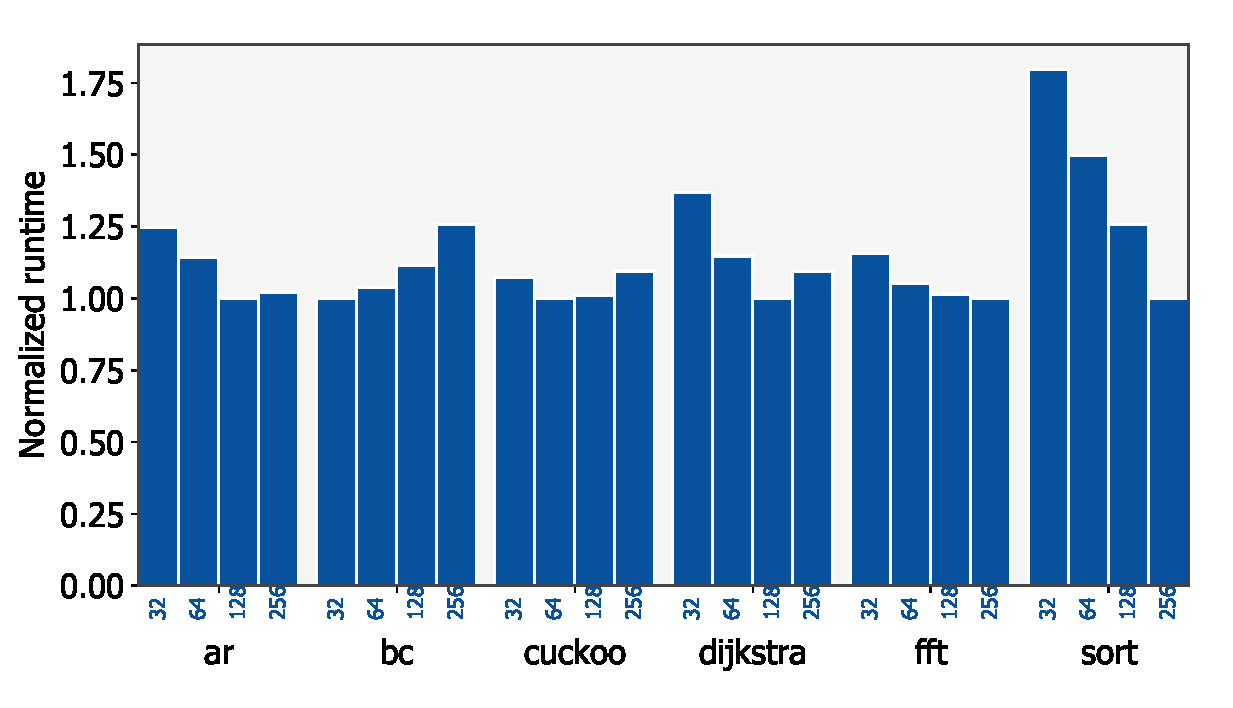
\includegraphics[width=\columnwidth]{figures/page_exec-time}
	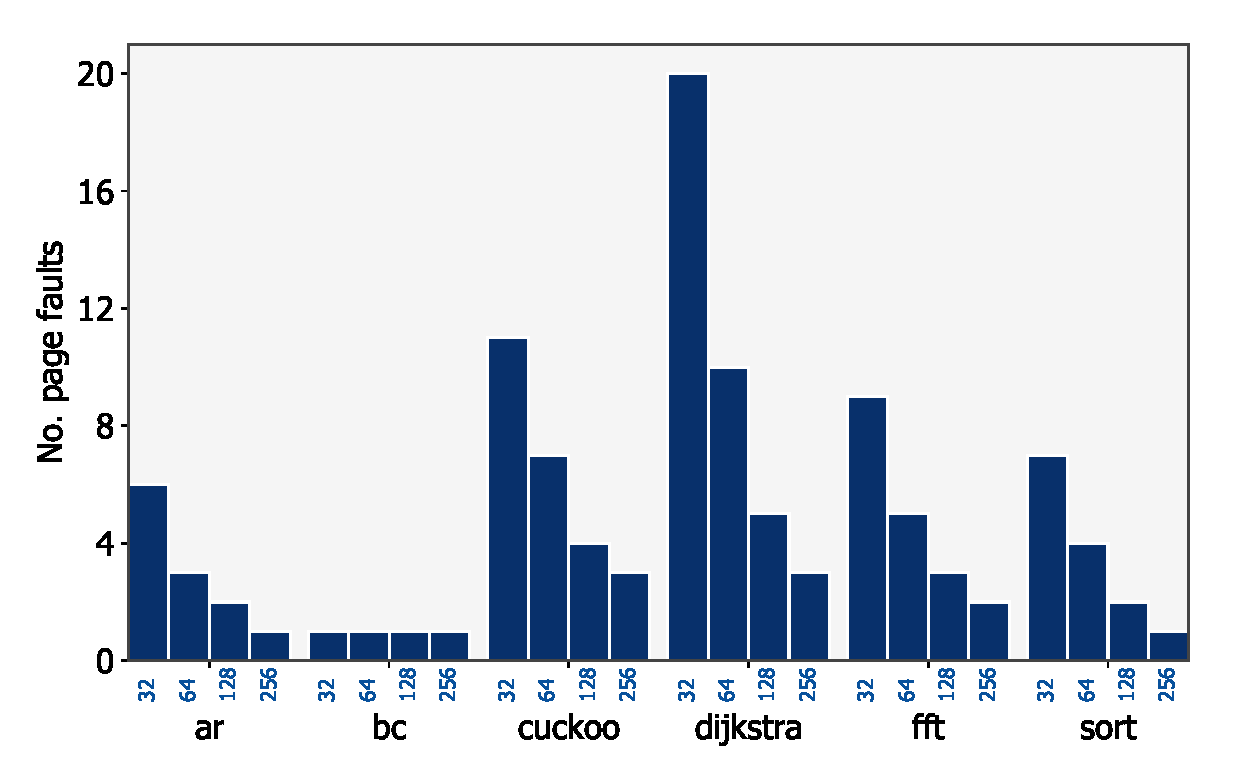
\includegraphics[width=\columnwidth]{figures/pagePulls}
	\caption{\textbf{\sys normalized runtime for various page sizes, \{32, 64,128,256\}\,bytes, per application (top) and respective page pulls (bottom)}).}\vspace{-0.5cm}
%\todo{change X to 0, remove the definition of X from caption}{Amjad}}
	\label{fig:page_size}
\end{figure}

\subsection{\sys Programs Characterization}
\label{sec:results_program_characterization}

\sys program characterization is provide in Table~\ref{table:compiler_result}. \todo{Finalize this section}{Przemek}

\begin{table}
	\begin{tabular}{| c | c | c | c | c |}
		\hline
		Application & \multicolumn{2}{| c |}{Memory footprint} & No. tasks & SLOC \\
		{} & \sys & Alpaca & {} & {} \\
		\hline\hline
		\textbf{ar} & --- & --- & --- & ---\\
		\hline
	\end{tabular}
		\caption{Comparison between \sys and Alpaca benchmarks.}
		\label{table:compiler_result}\vspace{-0.5cm}
\end{table}

%\begin{table}[t]
%	\centering
%	\renewcommand{\tabcolsep}{1pt}
%	\begin{tabular}{|l|cc|cc|cc|cc|c|}
%		\hline
%		{} & \multicolumn{2}{c|}{{\bf Prot. bytes}} & \multicolumn{2}{c|}{{\bf \# Tasks}} & \multicolumn{2}{c|}{{\bf \# Prot. acc.}} & \multicolumn{2}{c|}{\bf SLOC} & {\bf Comp.} \\
%		App & Man. & Comp. & Man. & Comp. & Man. & Comp. & \multicolumn{1}{l}{\sys} & \multicolumn{1}{r|}{Chain~\cite{chain}} & {\bf time} \\
%		\hline\hline
%		bc & 22 & 22 & 10 & 15 & 81 & 93 & 351 &588 & 3\\
%		cem & 3492 & 3242 & 12 & 9 & 92 & 123 & 388 &721 & 2\\
%		cuckoo & 282 & 288 & 15 & 6 & 90 & 76 & 483 &762 & 6\\
%		rsa & 332 & 250 & 20 & 27 & 130 & 296 & 887 &1233 & 86\\
%		ar & 166 & 218 & 11 & 6 & 112 & 333 & 483 &762 & 34\\
%		sort & 104 & 104 & 4 & 2 & 70 & 23 & 180 & 287 & $<$1\\
%		dft$^\dagger$ & --- & --- & --- & --- & --- & --- & 222 & 293 & ---\\
%		%dd &  &  &  &  &  &  &  & 287 &  \\
%		\hline
%	\end{tabular}
%		\caption{Comparison between \sys and Alpaca benchmarks.}
%		\label{table:compiler_result}\vspace{-0.5cm}
%\end{table}